

\subsection*{Le contexte général}
\noindent
%De quoi s'agit-il ? 
%D'où vient-il ? 
%Quels sont les travaux déjà accomplis dans ce domaine dans le monde ?
Un maillage représente un domaine géometrique en le discretisant en formes simples. Les maillages permettent de représenter des objets géométriques en 1, 2 ou 3D à des fins scientifiques ou industrielles par exemple. En 2D, les maillages representent des surfaces et sont constitués de polygones (triangles, carrés...) reliés deux à deux par une arête. On parle de maillages surfaciques. En 3D, les maillages représentent des volumes à l'aide de polyèdres (tétraèdres, pyramides...) partageant une face commune. On parle alors de maillages volumiques. Les maillages sont très utilisés pour la visualisation de volume, calculs de solutions pour des équations aux dérivées partielles... Cependant, ce sont des structures complexes qui peuvent devenir très volumineuses et dont on essaye de réduire la taille mémoire.

\subsection*{Le problème étudié}
\noindent
%Quelle est la question que vous avez abordée ? 
%Pourquoi est-elle importante, à quoi cela sert-il d'y répondre ?  
%Est-ce un nouveau problème ?
%Si oui, pourquoi êtes-vous le premier chercheur de l'univers à l'avoir posée ?
%Si non, pourquoi pensiez-vous pouvoir apporter une contribution originale ?
La compression de données est omniprésente en informatique, avec des formats compressés génériques comme \textit{gzip} mais aussi dédiés comme \textit{mp3} pour les fichiers audios. Ce besoin de compresser les données est grandissant car de plus en plus de fichiers sont stockés à distance sur des serveurs et la moindre économie de stockage a d'importantes répercussions. Néanmoins, sous certains formats compressés, les données originales deviennent inutilisables (ex : \textit{rar}). Cela pose problème quand l'on souhaite accéder aux données  sans passer par l'étape de décompression.\\
Une structure de données est une manière d'organiser les données pour faciliter leur traitement. Les listes, arbres et graphes sont des exemples de structures de données. Leur but n'est pas de limiter l'usage mémoire mais seulement de faciliter l'utilisation des données. Ainsi, pour certains formats volumineux, des structures de données compactes ont été inventées. Ce sont des structures de données compressées, c'est à dire des structures de données dont l'utilisation de la mémoire est limitée.\\
Si l'on revient aux maillages, les algorithmes de compression limitent au maximum l'usage mémoire du maillage et il devient alors inutilisable sous forme compressé tandis que la structure de données pré-traite le maillage en réduisant l'usage mémoire mais celui-ci reste utilisable.\\ 
Les maillages surfaciques sont majoritairement utilisés car ils sont plus léger, et permettent de représenter implicitement des volumes (la frontière). Par conséquent, de nombreuses structures de données compactes ont été créees afin de faciliter leur utilisation. Les maillages volumiques étant beaucoup moins utilisés pour l'instant, peu de structure de données compactes leur sont dévolues. Néanmoins, leur utilisation croissante incite à procéder de même. La suite de ce rapport sera principalement consacrée aux structures de données compactes pour maillages volumiques tétraèdriques.

\subsection*{La contribution proposée}
\noindent
De manière générale, un structure de données pour maillage stocke trois types d'informations :
\begin{itemize}
\item La géométrie, c'est à dire les positions des sommets
\item La connectivité, les relations d'adjacence entre les tétraèdres
\item Des attributs (par sommet, par arête, par face, par tétraèdre)\\
\end{itemize}
Elle doit par ailleurs supporter des requêtes simples :
\begin{itemize}
\item Quels sont les sommets de la ième face ?
\item Quel est le degré du ième sommet ?
\item Quelles sont les tétraèdres adjacents au ième tétraèdre ?
\item ...
\end{itemize}
%Par ailleurs, suivant l'utilisation ciblée, la structure de données devra être en mesure de satisfaire des opérations de modification :
%\begin{itemize}
%\item Ajouter/Enlever un sommet
%\item Ajouter/Enlever/Séparer un tetra\\
%\end{itemize}
Dans ce rapport, nous présentons une structure de données compacte permettant de représenter la connectivité d'un maillage tétraèdrique en utilisant en moyenne 2.4 références par tétraèdre. Le principe de notre structure consiste à regrouper les tétraèdres en diamants. Nous exploitons le fait que les tétraèdres puissent être ordonnés autour d'une arête. Cet ordre permet d'omettre des informations de connectivité. Notre structure de données permet l'accès au ième sommet, au ième tétraèdre en temps constant et à l'hypersphère d'un sommet en temps proportionnel au degré du sommet. Son implémentation est simple et l'utilisation d'un tableau d'entiers afin de représenter les références permet une interopérabilité entre les languages de programmation.

\subsection*{Les arguments en faveur de sa validité}
\noindent
Notre structure de données est en moyenne 40\% plus économique que la meilleure structure de données disponible actuellement pour les maillages tétraèdriques. Cette économie est purement empirique et nous n'apportons que peu de garanties théoriques concernant la place mémoire occupée par notre structure. La validité de la solution que nous proposons est directement liée aux expériences menées. Par conséquent, afin que nos résultats soient fidèles à la réalité, nous évaluons notre structure sur une dizaine de maillages aux propriétés différentes en prétant particulièrement attention au temps requis pour la construction, au temps nécessaire pour répondre à de simples requêtes et à la taille mémoire consommée.

\subsection*{Le bilan et les perspectives}
\noindent
Notre structure permet d'encoder de réduire la taille mémoire de la connectitivé du maillage sans utiliser sa géométrie. Par conséquent, cela rend notre approche très générale.\\
Néanmoins, notre structure de données est statique. Elle ne permet pas de modifier le maillage localement. Rendre notre structure dynamique en permettant l'ajout de sommets ou l'ajout de tétraèdres permettrait une utilisation encore plus étendue.\\
Par ailleurs, notre structure est destinée aux maillages tétraèdriques et plus particulièrement aux variétés tétraèdriques. Cependant, les maillages hexaèdriques sont souvent préférés aux maillages tétraèdriques car ils offrent un meilleur ratio entre précision et temps de calcul. Une autre piste de recherche intéressante serait donc l'extension de notre structure aux maillages hexaèdriques.

\subsection*{Remerciements}
\noindent
Je tiens à remercier mon superviseur Luca Castelli Aleardi pour sa précieuse aide ainsi que pour ses très intéressantes pistes de réflexion. Je remercie aussi Olivier Devillers pour ses explications des travaux effectués en compression de maillages.

\newpage
\section{Préliminaires}
\noindent
Ce rapport fait appel à des notions de géométrie. Afin que tous les termes employés soient compris par le lecteur, nous allons en définir certains qui seront employés tout au long de ce rapport.
\subsection{Définitions}
\noindent
\textbf{Simplexe}. Un simplex $\sigma^p$ de dimension $p$ est l'enveloppe convexe de $p+1$ points $\{v_0,v_1,...v_p\}$, où $v_i\, \in R^n$ et les vecteurs $v_1-v_0,v_2-v_0...$ sont linéairement indépendants. Les simplexes de dimensions 0, 1, 2 et 3 sont respectivement les sommets, arêtes, triangles et tétraèdres.\\\\
\textbf{Complexe simplicial}. Un complexe simplicial est un ensemble K de simplexes d'un espace affine tel que toutes les faces de chaque simplexe de K appartiennent aussi à K et si deux simplexes $\sigma$ et $\tau$ de K sont adjacents alors $\sigma \cap \tau \neq \emptyset$.\\\\
%Les points $v_0,v_1,...v_p$ sont appelés les sommets de $\sigma$. 
%Une face est l'enveloppe convexe d'une partie des sommets (pas tout). Si un simplex $\sigma$ est la face d'un simplexe $\tau$, alors $\tau$ est dit incident et $\tau$ limite $\sigma$. La frontière d'un p-simplexe $\sigma$ $\partial \sigma$ est la collection de toutes ses faces.\\\\
%\textbf{Etoile}. L'étoile ouverte d'un simplexe $\sigma \in K$ noté étoile($\sigma$,$K$) est l'union de tous les simplexes de l'étoile avec ses faces.\\\\
\textbf{Variété}. Une variété topologique (manifold en anglais) M de dimension n est un espace topologique connexe séparé localement homéomorphe à un ouvert de $\mathbb{R}^n$. C'est à dire que chaque point de M admet un voisinage homéomorphe à un ouvert de $\mathbb{R}^n$.\\\\
\textbf{Variété à bord}. Une variété à bord est un sous-espace topologique dont les points admettent un voisinage homéomorphe à $\mathbb{R}^n$ (les points intérieurs) ou un voisinage homéomorphe à $\mathbb{R}^{n-1}  $x$ \mathbb{R}^+$ (les points bordants). L'ensemble des points bordants constitue le bord de la variété.\\\\
\textbf{Frontière}. Les (k-1)-simplexes d'une k-variété M qui sont incidents à seulement un k-simplexe sont les simplexes frontières. L'ensemble des simplexes frontières est dénoté $\partial $M.\\\\
%Une k-variété est orientable s'il est possible de choisir une orientation cohérente pour tout ses simplexes. Une orientation est cohérente si deux k-faces adjacentes induisent deux orientations opposées sur leur (k-1)-face.
%Un complexe simplicial  $M$ est une k-variété si l'étoile ouverte d'un sommet dans $M$ est homeomorphique à $R^k$ ou à $R^{k-1}XR_+$. En particulier, si $M$ est une variété alors tout (k-1)-simplex dans $M$ est la frontière de un ou deux k-simplexe.\\
\textbf{Maillage}. Un maillage est un complexe simplicial représentant un objet géométrique. Il a la même dimension que l'objet qu'il représente. Ainsi, pour tout objet en 1, 2 ou 3D, les maillages respectifs seront en dimensions 1, 2 ou 3. Dans un maillage de dimension d, les simplexes de dimensions (d-1) sont appelées des facettes. Ainsi, les facettes d'un tétraèdre sont ses faces, les facettes d'une face sont ses arêtes et les facettes d'une arête sont ses sommets.\\\\
\textbf{Le degré}. Le degré d'un k-simplexe est le nombre de (k+1)-simplexes adjacents. Ainsi le degré d'un sommet est le nombre d'arêtes adjacentes et le degré d'une arête est le nombre de faces adjacentes.\\\\
\textbf{Etoile}. L'étoile d'un sommet est l'ensemble des k-simplexes adjacents à un sommet. C'est l'ensemble des triangles (resp. tétraèdres) adjacents à un sommet dans le cas surfacique (resp. volumique). Dans ce dernier cas, on appelle cela l'hypersphère.

%Nous traitons dans ce rapport de maillages tetrahedriques dans un espace Euclidien à 3 dimensions. Deux tetrahedres sont dit adjacents s'ils partagent une face. On dénote par V l'ensemble des sommets, E l'ensemble des arêtes, F l'ensemble des faces et T l'ensemble des tetrahedres du maillage.\\
%En utilisant l'équation d'Euler, on a la relation suivante : 
%\begin{equation}
%|V|-|E|+|F|-|T|=\chi
%\end{equation}

\subsection{Combinatoire}
\noindent
%Les maillages dont nous allons parler dans la suite de ce rapport sont avant tout des complexes simpliciaux dont la combinatoire des simplexes est étudiée depuis de nombreuses années. 
En mathématique et en optimisation combinatoire, la caractéristique d'Euler $\chi$ est un invariant topologique décrivant la forme d'un objet géométrique. Par conséquent, la valeur de $\chi$ ne change pas après déformation continue de l'objet géométrique.
\begin{equation}
\chi = \sum_{i=0} (-1)^i \, |dim(H_i)| = 2-2g
\end{equation}
\begin{itemize}
\item $H_i$ est l'ensemble des faces de dimension $i$
\item $g$ est le genre (le nombre de trou de l'objet étudié)\\ 
\end{itemize}

\begin{figure}[th]
\centering
\begin{subfigure}{.5\textwidth}
  \centering
  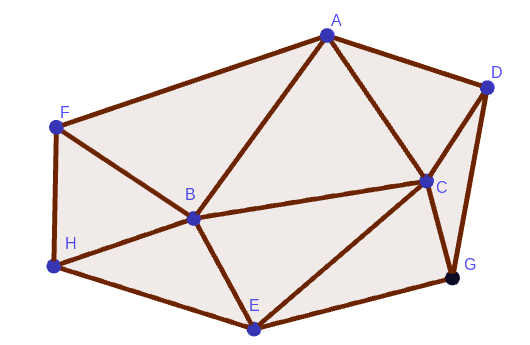
\includegraphics[scale=0.3]{Images/planar_graph}
\end{subfigure}%
\begin{subfigure}{.5\textwidth}
  \centering
  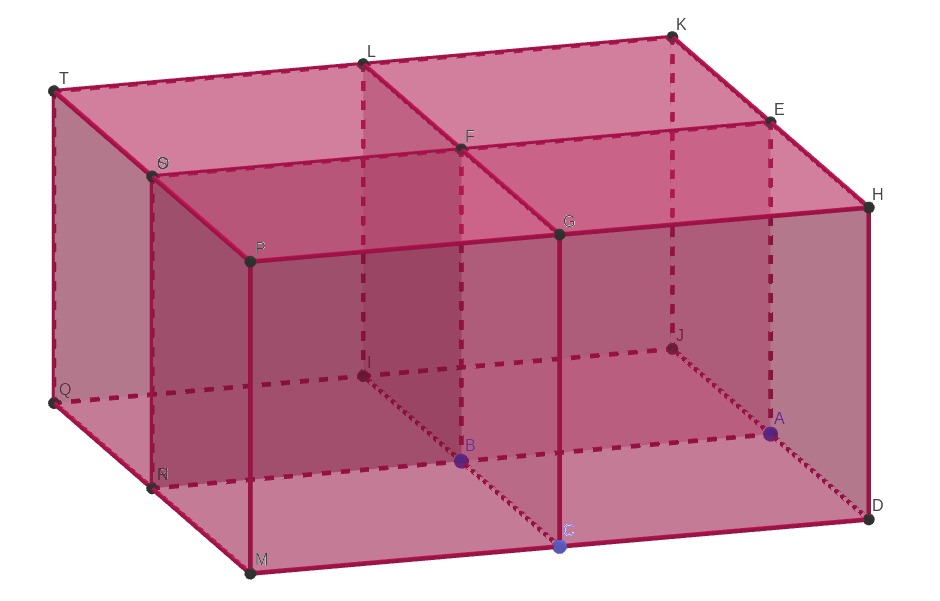
\includegraphics[scale=0.18]{Images/4cubes}
\end{subfigure}
\caption{\textbf{Gauche} : Graphe planaire ($|V|=8$,$|E|=15$,$|F|=9$). \textbf{Droite} : Polyèdre ($|V|=18$,$|E|=33$,$|F|=20$,$|T|=4$)}
\label{fig:planar_graph_4cubes}
\end{figure}
\noindent

\subsubsection{Cas surfacique}
\label{combi_2d}
\noindent
Dans le cas surfacique, la formule devient :
\begin{equation}
\label{eq:euler_surfacique}
\chi = |V|-|E|+|F|
\end{equation}
\begin{itemize}
\item $V$ est l'ensemble des sommets
\item $E$ est l'ensemble des arêtes
\item $F$ est l'ensemble des faces (ie. polygones)\\
\end{itemize}
Si nous sommes dans le cadre d'une triangulation surfacique et sans trou, alors chaque face est bordée par 3 arêtes et chaque arête n'étant par sur les bords appartient à 2 faces. Par conséquent $3F\leqslant 2E$. Ainsi l'équation \ref{eq:euler_surfacique} devient :\\
\begin{align*}
2 &\leqslant |V| - |E| + \frac{2}{3}|E| = |V| - \frac{1}{3}|E|\\
|E|&\leqslant 3|V|-6
\end{align*}
Il y a donc dans une triangulation surfacique environ 3 fois plus d'arêtes que de sommets.
\subsubsection{Cas volumique}
\noindent
Pour un maillage volumique, la formule d'Euler contient un terme de plus :\\
\begin{equation}
\chi = |V|-|E|+|F|-|T|
\end{equation}
\begin{itemize}
\item $T$ est l'ensemble des polyèdres (tétraèdres, hexaèdres...)\\
\end{itemize}
Si l'objet considéré est une variété alors chaque facette qui n'est pas sur les bords du volume est partagée par deux polyèdres, alors :\\
\begin{equation}
|F|\simeq 2|T|
\end{equation}
Ainsi :
\begin{equation}
\chi \simeq |V|-|E|+|T|
\end{equation}
Il y a donc autant d'arêtes que de polyèdres et sommets réunis (Tab. \ref{tab:caract_maillages}).

\subsection{Représentation des maillages tétraèdriques}
\label{representation_maillages_tetra}
\noindent
Ce rapport se concentre sur les structures de données pour maillages tétraèdriques. Comme rappelé dans l'introduction, une structure de données doit fournir une implémentation des opérateurs permettant la navigation et l'accès à la combinatoire du maillage (décrite par les relations d'incidence entre ses éléments). Dans le cas de maillages tétraèdriques, il est usuel de disposer des opérations suivantes:
\begin{itemize}
\item \texttt{incident\_face($i,t$)}: renvoie la $i$-ème face du tétraèdre $t$ (pour $i=0..3$).
\item \texttt{incident\_vertex($v$)}: renvoie un des tétraèdres incidents au sommet $v$.
\item \texttt{neighbour($i, t$)}: renvoie le tétraèdre qui est le $i$-ème voisin adjacent au tétraèdre $t$. 
\item \texttt{get\_vertex\_index($v,t$)}: renvoie un entier $i\in\{0 \ldots 3 \}$, l'indice du sommet $v$ dans le tétraèdre $t$.
%\indent \texttt{degree(i)} Cette fonction doit permettre de calculer le degré d'un sommet\\
%\indent \texttt{hypersphere(i)} Cette fonction doit retourner l'hypersphère ou l'étoile d'un sommet, c'est à dire l'ensemble des tétraèdres possédant le ième sommet.\\
%\indent \texttt{breadth\_first\_search(t)} Cette fonction doit permettre de réaliser un parcours en largeur du maillage en commen\c cant par le tétraèdre t .\\
\end{itemize}
\noindent
La combinaison de ces fonctions permet de réaliser la quasi-totalité des opérations de navigation locale qui sont effectuées habituellement
dans le cadre des procédures de modélisation géométrique et géométrie algorithmique. A titre d'exemple, on peut implémenter de manière efficace les fonctions suivantes:
\begin{itemize}
\item \texttt{degree($v$)}: renvoie le degré d'un sommet $v$
\item \texttt{hypersphere($v$)}: renvoie l'hypersphère ou l'étoile d'un sommet $v$, c'est à dire l'ensemble des tétraèdres incidents à $v$.
\item \texttt{BFS($t$)}: réalise un parcours en largeur du maillage en commen\c cant par le tétraèdre $t$.
\end{itemize}
On dit que la structure de données est \emph{indexable} si, de plus, elle permet l'accès en temps constant aux éléments du maillage (ses faces, sommets, ...), par le biais des opérations suivantes:
\begin{itemize}
\item \texttt{tetrahedron($i$)}: donne accès au $i$-ème tétraèdre,
\item \texttt{vertex($i$)}: donne accès au $i$-ème sommet.
\end{itemize}
Ces deux opérations sont parfois importantes dans plusieurs applications: elles permettent, par exemple, d'itérer sur tous les sommets ou tétraèdres,
ainsi que de récupérer les attributs qui y sont associés (couleurs, normales, coordonnées, ...).

\paragraph{Implantation naïve}
Une solution simple à implémenter (utilisée, entre autres, par la librarie \texttt{CGAL}~\cite{CGAL}) permettant de représenter un maillage tétraèdrique consiste à stocker explicitement les relations d'adjacence entre tétraèdres voisins et les relations d'incidence tétraèdre/sommet. Plus précisément,  on stocke pour chaque tétraèdre plusieurs références : 
\begin{itemize}
\item $4$ références par tétraèdre donnant l'accès aux tétraèdres voisins
\item $4$ références par tétraèdre donnant l'accès aux sommets incidents
\item $1$ référence par sommet donnant l'accès à l'un de ses tétraèdres incidents
\end{itemize}
Au total, on comptabilise donc $8$ références par tétraèdre et $1$ référence par sommet ($8|T|+|V|$)~\footnote{Lorsqu'on parle de références il peut s'agir, selon le langage de programmation et environnement de travail choisi, de pointeurs (comme en \texttt{C/C++}), 
de références (comme en \texttt{Java}), ou d'indices si l'implémentation mise en place fait appel à des tableaux d'entiers (dans ce cas une référence vers un tétraèdre co\^utera
$\lceil\log_2 |T|\rceil$ bits).}.